\documentclass{beamer}
\usetheme{metropolis}
\usepackage{graphicx}
\usepackage{subfig}
\usepackage{tcolorbox}
\title{Calculus-Based Physics-2: Electricity, Magnetism, and Thermodynamics (PHYS180-02): Unit 3}
\author{Jordan Hanson}
\institute{Whittier College Department of Physics and Astronomy}

\begin{document}
\maketitle

\section{Summary}

\begin{frame}{Unit 3 Summary}
\textbf{Reading: Chapter 11 and 12}
\begin{enumerate}
\item Magnetism and magnetic fields
\item Motion of a charged particle in a magnetic field
\item Forces on conductors carrying current
\item Current loops
\item The Hall effect
\item Applications
\item Amp\`{e}re's Law
\end{enumerate}
\end{frame}

\section{Magnetism and magnetic fields}

\begin{frame}{Magnetism and magnetic fields}
\begin{figure}
\centering
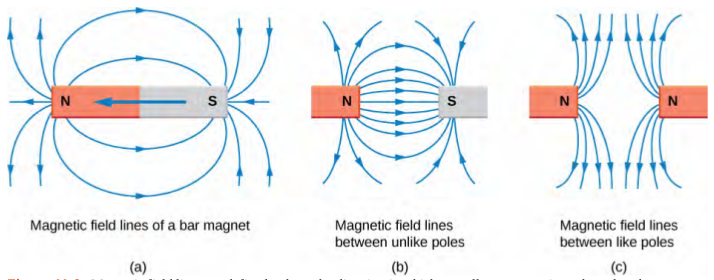
\includegraphics[width=0.9\textwidth,trim=0cm 1cm 0cm 0cm,clip=true]{figures/fields1.png}
\caption{\label{fields1} Various magnetic field line configurations.}
\end{figure}
\end{frame}

\begin{frame}{Magnetism and magnetic fields}
\begin{figure}
\centering
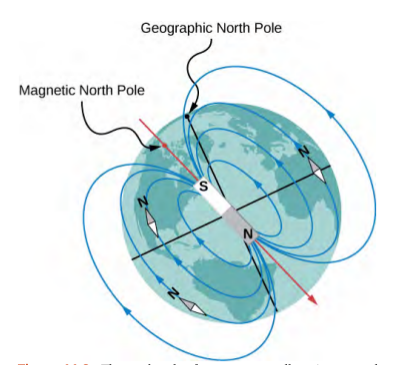
\includegraphics[width=0.6\textwidth,trim=0cm 0.1cm 0cm 0cm,clip=true]{figures/fields2.png}
\caption{\label{fields2} The magnetic and geographic poles are not the same.}
\end{figure}
\end{frame}

\begin{frame}{Magnetism and magnetic fields}
It would be nice if we could say:
\begin{equation}
F = \mu_0 \frac{q_{m,1} q_{m,2}}{r^2}
\end{equation}
But...we can't.  Why?  There's no such thing has magnetic charge:
\begin{align}
\nabla \cdot \vec{E} &= \rho/\epsilon_0 \\ 
\nabla \cdot \vec{B} &= 0
\end{align}
But there is a force associating charge and magnetic fields.  But first, let's review the cross-product.
\end{frame}

\begin{frame}{Magnetism and magnetic fields}
What is a cross-product and how does it work? \\ \vspace{0.25cm}
\begin{figure}
\centering
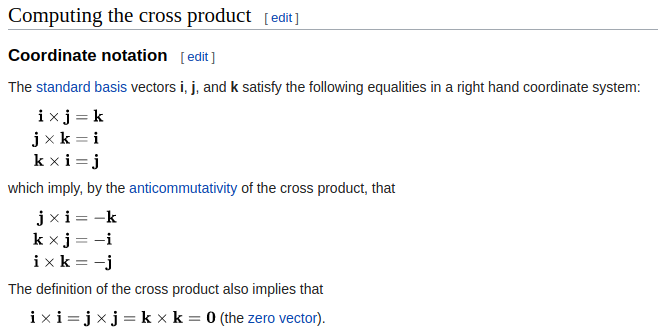
\includegraphics[width=0.75\textwidth]{figures/crossP.png}
\caption{\label{fig:crossP} The cross-product is a way of multiplying unit vectors.}
\end{figure}
\textbf{Examples:} (i) Working with unit vectors (ii) Working with two-dimensional vectors (iii) A three-dimensional example.
\end{frame}

\begin{frame}{Magnetism and magnetic fields}
Let $\vec{v} = 2\hat{i}$ and $w = -2 \hat{j}$.  What is $\vec{v} \times \vec{w}$?
\begin{itemize}
\item A: $-4 \hat{k}$
\item B: $4 \hat{k}$
\item C: $-2 \hat{i}$
\item D: $2 \hat{j}$
\end{itemize}
\end{frame}

\begin{frame}{Magnetism and magnetic fields}
Let $\vec{v} = 3\hat{j}$ and $w = 5 \hat{k}$.  What is $\vec{v} \times \vec{w}$?
\begin{itemize}
\item A: $15 \hat{i}$
\item B: $5 \hat{j}$
\item C: $3 \hat{i}$
\item D: $15 \hat{k}$
\end{itemize}
\end{frame}

\begin{frame}{Magnetism and magnetic fields}
Let $\vec{v} = 3\hat{i} + 3\hat{j}$ and $w = 2 \hat{k}$.  What is $\vec{v} \times \vec{w}$?
\begin{itemize}
\item A: $-6 \hat{j} + 6\hat{k}$
\item B: $-6 \hat{j} + 6\hat{i}$
\item C: $6 \hat{j} + 6\hat{i}$
\item D: $6 \hat{k} + 6\hat{i}$
\end{itemize}
\end{frame}

\begin{frame}{Magnets and magnetic fields}
\textbf{Group exercise:} Compute the following cross product:
\begin{align}
\vec{v} &= 2\hat{i}-2\hat{j} \\
\vec{w} &= 4\hat{j}-4\hat{i} \\
\vec{v} \times \vec{w} &= ??
\end{align}
\textit{What happens when we draw these two vectors?}
\end{frame}

\begin{frame}{Magnets and magnetic fields}
\textbf{Group exercise:} Compute the following cross product:
\begin{align}
\vec{v} &= 2\hat{i}-2\hat{j}+\hat{k} \\
\vec{w} &= 4\hat{j}-4\hat{i}-\hat{k} \\
\vec{v} \times \vec{w} &= ??
\end{align}
\textit{Use your knowledge of unit vectors to skip the terms that are zero.}
\end{frame}

\begin{frame}{Magnets and magnetic fields}
\begin{tcolorbox}[colback=white,colframe=black!40!black,title=The Lorentz Force]
\alert{Let a particle with charge q and velocity $\vec{v}$ move through a magnetic field $\vec{B}$. The Lorentz force on the charged particle is
\begin{equation}
\vec{F}_{\rm L} = q\vec{v} \times \vec{B}
\label{eq:Lorentz}
\end{equation}}
\end{tcolorbox}
\textit{As a helpful memory tool, we have the right-hand rule to
remember the direction of the cross-product.} The units of the
magnetic field are the Telsa, after Nikola Tesla. We also have
the Gauss which is $10^{-4}$ Tesla.
\end{frame}

\begin{frame}{Magnets and magnetic fields}
\begin{figure}
\centering
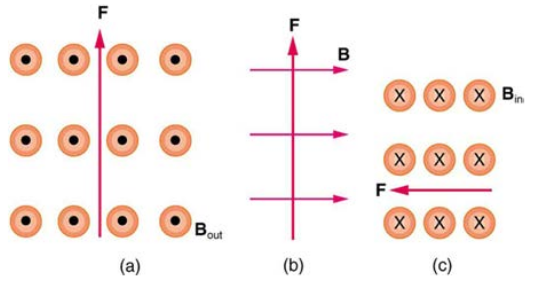
\includegraphics[width=0.75\textwidth]{figures/lorentzProblem.png}
\caption{\label{fig:lorentzProblem} Three different magnetic field and charge scenarios. The
vector $\vec{F}$ is the direction of the Lorentz force, and the magnetic field
is uniform. A dot indicates that the magnetic field is coming out of
the page, and an x indicates that the field is going into the page.}
\end{figure}
\end{frame}

\begin{frame}{Magnets and magnetic fields}
\begin{columns}[T]
\begin{column}{0.3\textwidth}
In which of the diagrams is a positively charged particle moving to the left?
\begin{itemize}
\item A: A
\item B: B
\item C: C
\item D: WAT WAT WAT
\end{itemize}
\end{column}
\begin{column}{0.7\textwidth}
\begin{figure}
\centering
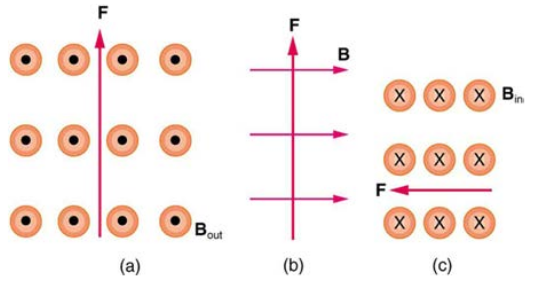
\includegraphics[width=0.75\textwidth]{figures/lorentzProblem.png}
\caption{\label{fig:lorentzProblem2} Three different magnetic field and charge scenarios.}
\end{figure}
\end{column}
\end{columns}
\end{frame}

\begin{frame}{Magnets and magnetic fields}
\begin{columns}[T]
\begin{column}{0.3\textwidth}
In which of the diagrams is a positively charged particle moving upwards?
\begin{itemize}
\item A: A
\item B: B
\item C: C
\item D: WAT WAT WAT
\end{itemize}
\end{column}
\begin{column}{0.7\textwidth}
\begin{figure}
\centering
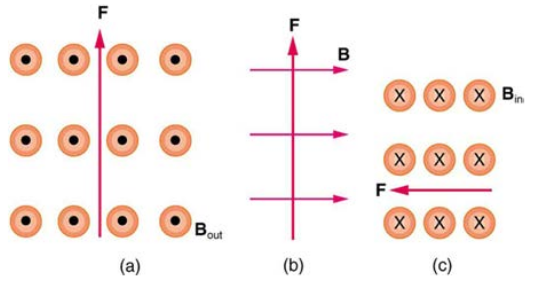
\includegraphics[width=0.75\textwidth]{figures/lorentzProblem.png}
\caption{\label{fig:lorentzProblem3} Three different magnetic field and charge scenarios.}
\end{figure}
\end{column}
\end{columns}
\end{frame}

\begin{frame}{Magnets and magnetic fields}
\begin{columns}[T]
\begin{column}{0.3\textwidth}
In which of the diagrams is a negatively charged particle moving into the page?
\begin{itemize}
\item A: A
\item B: B
\item C: C
\item D: WAT WAT WAT
\end{itemize}
\end{column}
\begin{column}{0.7\textwidth}
\begin{figure}
\centering
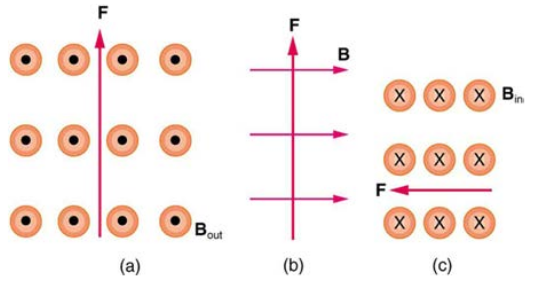
\includegraphics[width=0.75\textwidth]{figures/lorentzProblem.png}
\caption{\label{fig:lorentzProblem4} Three different magnetic field and charge scenarios.}
\end{figure}
\end{column}
\end{columns}
\end{frame}

\begin{frame}{Magnets and magnetic fields}
\begin{columns}[T]
\begin{column}{0.3\textwidth}
In which of the diagrams is a negatively charged particle moving to the right?
\begin{itemize}
\item A: A
\item B: B
\item C: C
\item D: WAT WAT WAT
\end{itemize}
\end{column}
\begin{column}{0.7\textwidth}
\begin{figure}
\centering
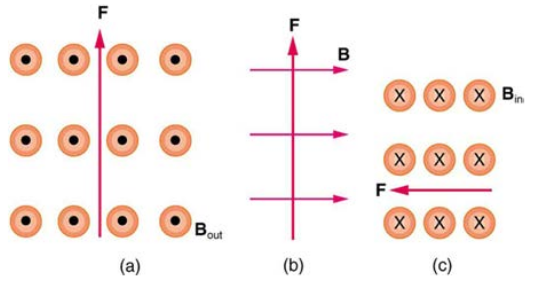
\includegraphics[width=0.75\textwidth]{figures/lorentzProblem.png}
\caption{\label{fig:lorentzProblem5} Three different magnetic field and charge scenarios.}
\end{figure}
\end{column}
\end{columns}
\end{frame}

\begin{frame}{Magnets and magnetic fields}
A theorem for the magnitude of the cross-product:  Let $\vec{a}$ and $\vec{b}$ be vectors and $\theta$ be the angle between them.  The magnitude of the cross product is:
\begin{equation}
|\vec{a} \times \vec{b}| =  a b \sin\theta
\end{equation}
Thus, the magnitude of the Lorentz force is
\begin{equation}
F_{\rm L} = q v B \sin\theta
\end{equation}
The angle $\theta$ is between the velocity and the magnetic field.
\end{frame}

\begin{frame}{Magnets and magnetic fields}
A cosmic ray proton moving toward the Earth at $3 \times 10^{6}$ m/s experiences a magnetic force of $2 \times 10^{-17}$ N. What is the strength of the magnetic field of the Earth? (1 Gauss = $10^{-4}$ Tesla).
\begin{itemize}
\item A: 0.1 Gauss
\item B: 0.6 Gauss
\item C: 1 Gauss
\item D: 6 Gauss
\end{itemize}
\end{frame}

\begin{frame}{Magnets and magnetic fields}
\begin{figure}
\centering
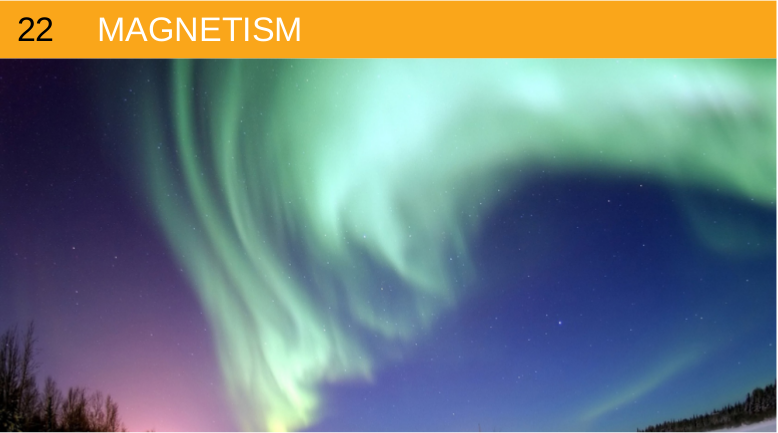
\includegraphics[width=0.9\textwidth]{figures/aurora.png}
\caption{\label{fig:aurora} The aurora borealis, or northern lights.}
\end{figure}
\end{frame}

\begin{frame}{Magnets and magnetic fields}
\begin{figure}
\centering
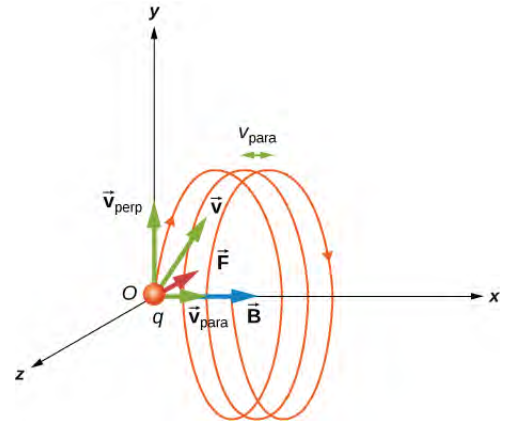
\includegraphics[width=0.5\textwidth]{figures/helix.png}
\caption{\label{fig:helix} In three dimensions, charged particle motion in a $\vec{B}$-field can result in \textit{helical motion}.}
\end{figure}
\end{frame}

\begin{frame}{Magnets and magnetic fields}
Suppose the velocity of a charged particle with mass $m$ is $\vec{v} = v_x \hat{i} + v_z \hat{k}$ through a uniform field $\vec{B} = B\hat{k}$.  The Lorentz force causes centripetal motion and the particle continues to have constant velocity in the $\hat{k}$ direction:
\begin{align}
\vec{F} &= q \vec{v} \times \vec{B} \\
\vec{F} &= -q B v_x \hat{j} \\
\frac{m v_x^2}{r} &= q B v_x \\
\omega &= \frac{v_x}{r} \\
\frac{q}{m} &= \frac{\omega}{B}
\end{align}
\textit{Sub-atomic properties are isolated!}
\end{frame}

\begin{frame}{Magnets and magnetic fields}
Which of the following is true of a charged particle moving in a helical fashion through a magnetic field?
\begin{itemize}
\item A: Raising the strength of the B-field increases the period
\item B: Raising the strength of the B-field increases the frequency
\item C: The particle has a constant velocity parallel to the field
\item D: B and C
\end{itemize}
\end{frame}

\begin{frame}{Magnets and magnetic fields}
Two unknown particles are moving in helixes through a region where there is a magnetic field.  One moves clockwise as you observe it, and the other moves counter-clockwise, and the helices have about the same radius.  Which of the following is true?
\begin{itemize}
\item A: The particles have identical charge.
\item B: The particles have identical charge, and the same mass.
\item C: The particles have opposite charge, and the same mass.
\item D: The particles have different masses.
\end{itemize}
\end{frame}

\begin{frame}{Magnets and magnetic fields}
Two unknown particles are moving in helixes through a region where there is a magnetic field.  Both move clockwise as you observe them. One particle spins around the field line with higher frequency compared to the other.  Which of the following is true?
\begin{itemize}
\item A: The particles are identical; they just had different initial conditions.
\item B: The charge is smaller for the particle with the larger frequency.
\item C: The mass is larger for the particle with the larger frequency.
\item D: The $q/m$ ratio is larger for the particle with the larger frequency.
\end{itemize}
\end{frame}

\begin{frame}{Magnets and magnetic fields}
\textbf{Group exercise}: Suppose we place a gas of unknown particles in the uniform magnetic field of Fig. \ref{fig:helix} and get them moving in a circle.  The angular frequency is 95.5788 MHz, and the B-field is exactly 1.0 T.  (a) Show that the relationship between the angular frequency $\omega$, the B-field strength $B$, and the $q/m$ ratio is $q/m = \omega/B$. (b) With which particle are we dealing?  Is it a proton, a neutron, an electron, or an alpha particle? (\textit{Hint: use the angular frequency and magnetic field to obtain the $q/m$ ratio, and then look up the masses and charges of these particles to make the determination}).
\end{frame}

\begin{frame}{Magnets and magnetic fields}
\textbf{Other examples:}
\begin{enumerate}
\item Magnetic fields do no work
\item Velocity selector
\item Mass spectrometer
\end{enumerate}
\end{frame}

\begin{frame}{Magnets and magnetic fields}
\begin{figure}
\centering
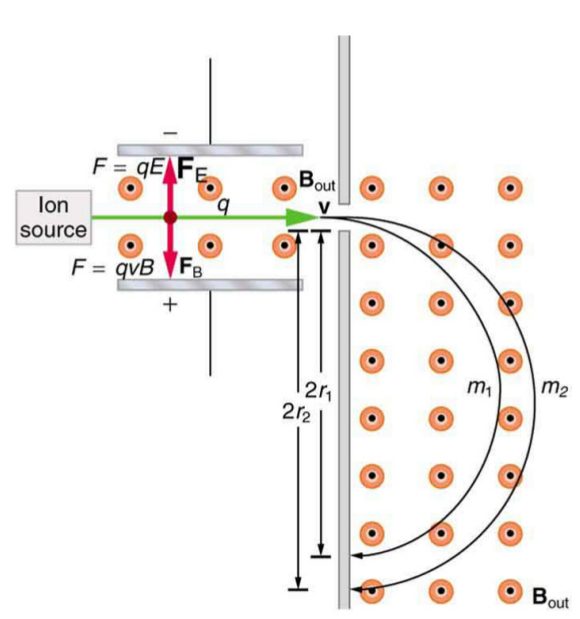
\includegraphics[width=0.5\textwidth]{figures/massspec.png}
\caption{\label{fig:massspec} The basic ideas behind a mass spectrometer.}
\end{figure}
\end{frame}

\begin{frame}{Magnets and magnetic fields}
\begin{figure}
\centering
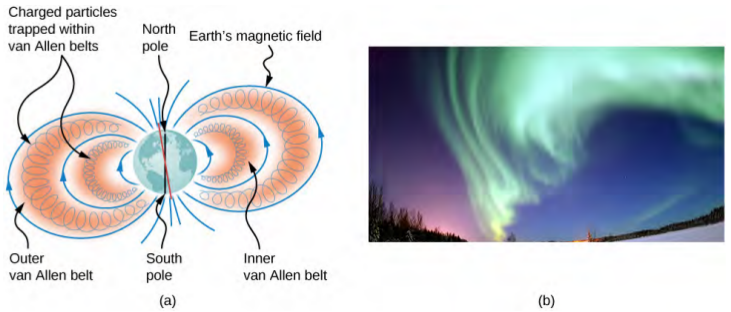
\includegraphics[width=0.85\textwidth]{figures/borealis.png}
\caption{\label{fig:borealis} We observe this effect in the auroras, and the van Allen belts.}
\end{figure}
\end{frame}

\begin{frame}{Magnets and magnetic fields}
A cool talk on the aurora borealis:
\url{https://youtu.be/czMh3BnHFHQ} \\
\begin{figure}
\centering
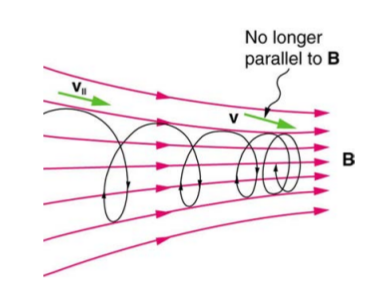
\includegraphics[width=0.45\textwidth]{figures/mag1.png}
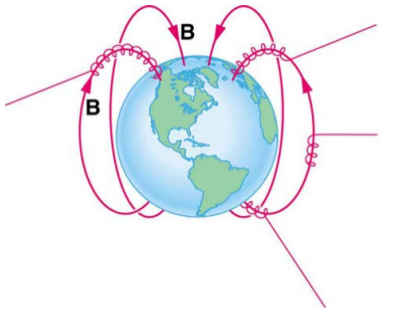
\includegraphics[width=0.45\textwidth]{figures/mag2.png}
\end{figure}
One un-explained piece: what does it mean for the electrons and protons to \textit{high-five} the neutral oxygen and nitrogen atoms?
\end{frame}

\section{Forces on Current-Carrying Conductors}

\begin{frame}{Forces on Current-Carrying Conductors}
Introductions to observable magnetic forces (PBS): \\ \vspace{1cm}
First connection between electricity and magnetism: \url{https://youtu.be/s94suB5uLWw} \\ \vspace{1cm}
Further experiments, Amp\`{e}re's Law: \url{https://youtu.be/5fqwJyt4Lus} \\ \vspace{1cm}
\end{frame}

\begin{frame}{Forces on Current-Carrying Conductors}
The Lorentz force, when applied to a section of current-carrying wire, becomes
\begin{equation}
d\vec{F} = I \vec{dl} \times \vec{B}
\end{equation}
\begin{figure}
\centering
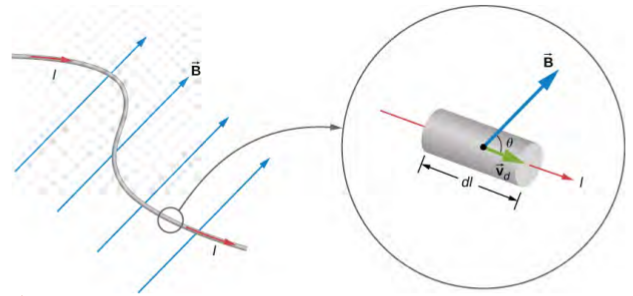
\includegraphics[width=0.55\textwidth]{figures/current.png}
\caption{\label{fig:current} The magnetic force on a section of current.}
\end{figure}
If the field is uniform:
\begin{equation}
\vec{F} = I \vec{L} \times \vec{B}
\end{equation}
\end{frame}

\begin{frame}{Forces on Current-Carrying Conductors}
\small
\textbf{Group exercise}: A wire of length 10 cm and mass 1 g is suspended in a horizontal plane by a pair of flexible leads.  The wire is then subjected to a constant magnetic field of magnitude 0.1 T, which is directed into the board.  What are the magnitude and direction of the current in the wire needed to remove the tension in the supporting leads?
\begin{figure}
\centering
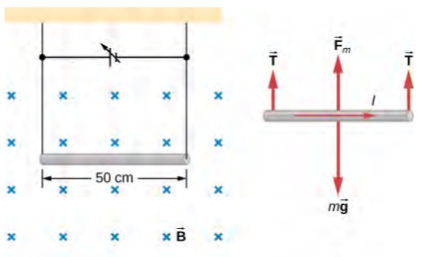
\includegraphics[width=0.5\textwidth]{figures/leads.png}
\caption{\label{fig:leads} Current suspended by Lorentz force...?}
\end{figure}
\end{frame}

\begin{frame}{Forces on Current-Carrying Conductors}
Suppose a power supply provides the current in the previous example.  What if the voltage is raised, and the resistance stays constant, so that the current is doubled.  What will happen?
\begin{itemize}
\item A: The wire will rise.
\item B: The wire will fall.
\item C: The magentic field will decrease.
\item D: Nothing.
\end{itemize}
\end{frame}

\begin{frame}{Forces on Current-Carrying Conductors}
If the wire rises, what is doing the work to raise it?
\begin{itemize}
\item A: The B-field
\item B: The current
\item C: The battery
\item D: Gravity
\end{itemize}
\end{frame}

\begin{frame}{Forces on Current-Carrying Conductors}
\small
\textbf{Group exercise}: Suppose the current is raised from 1 amp to 2 amps for 0.1 seconds.  By how much will the wire be raised?  \textit{Hint: you can obtain the acceleration from the \textbf{net} force, and then obtain the displacement.}
\begin{figure}
\centering
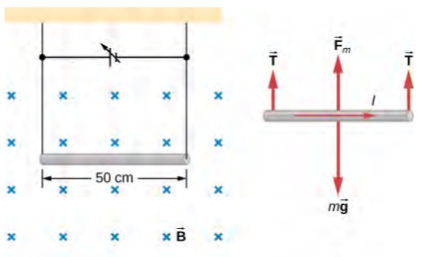
\includegraphics[width=0.5\textwidth]{figures/leads.png}
\caption{\label{fig:leads2} Current suspended by Lorentz force...?}
\end{figure}
\end{frame}

\begin{frame}{Forces on Current-Carrying Conductors}
\begin{figure}
\centering
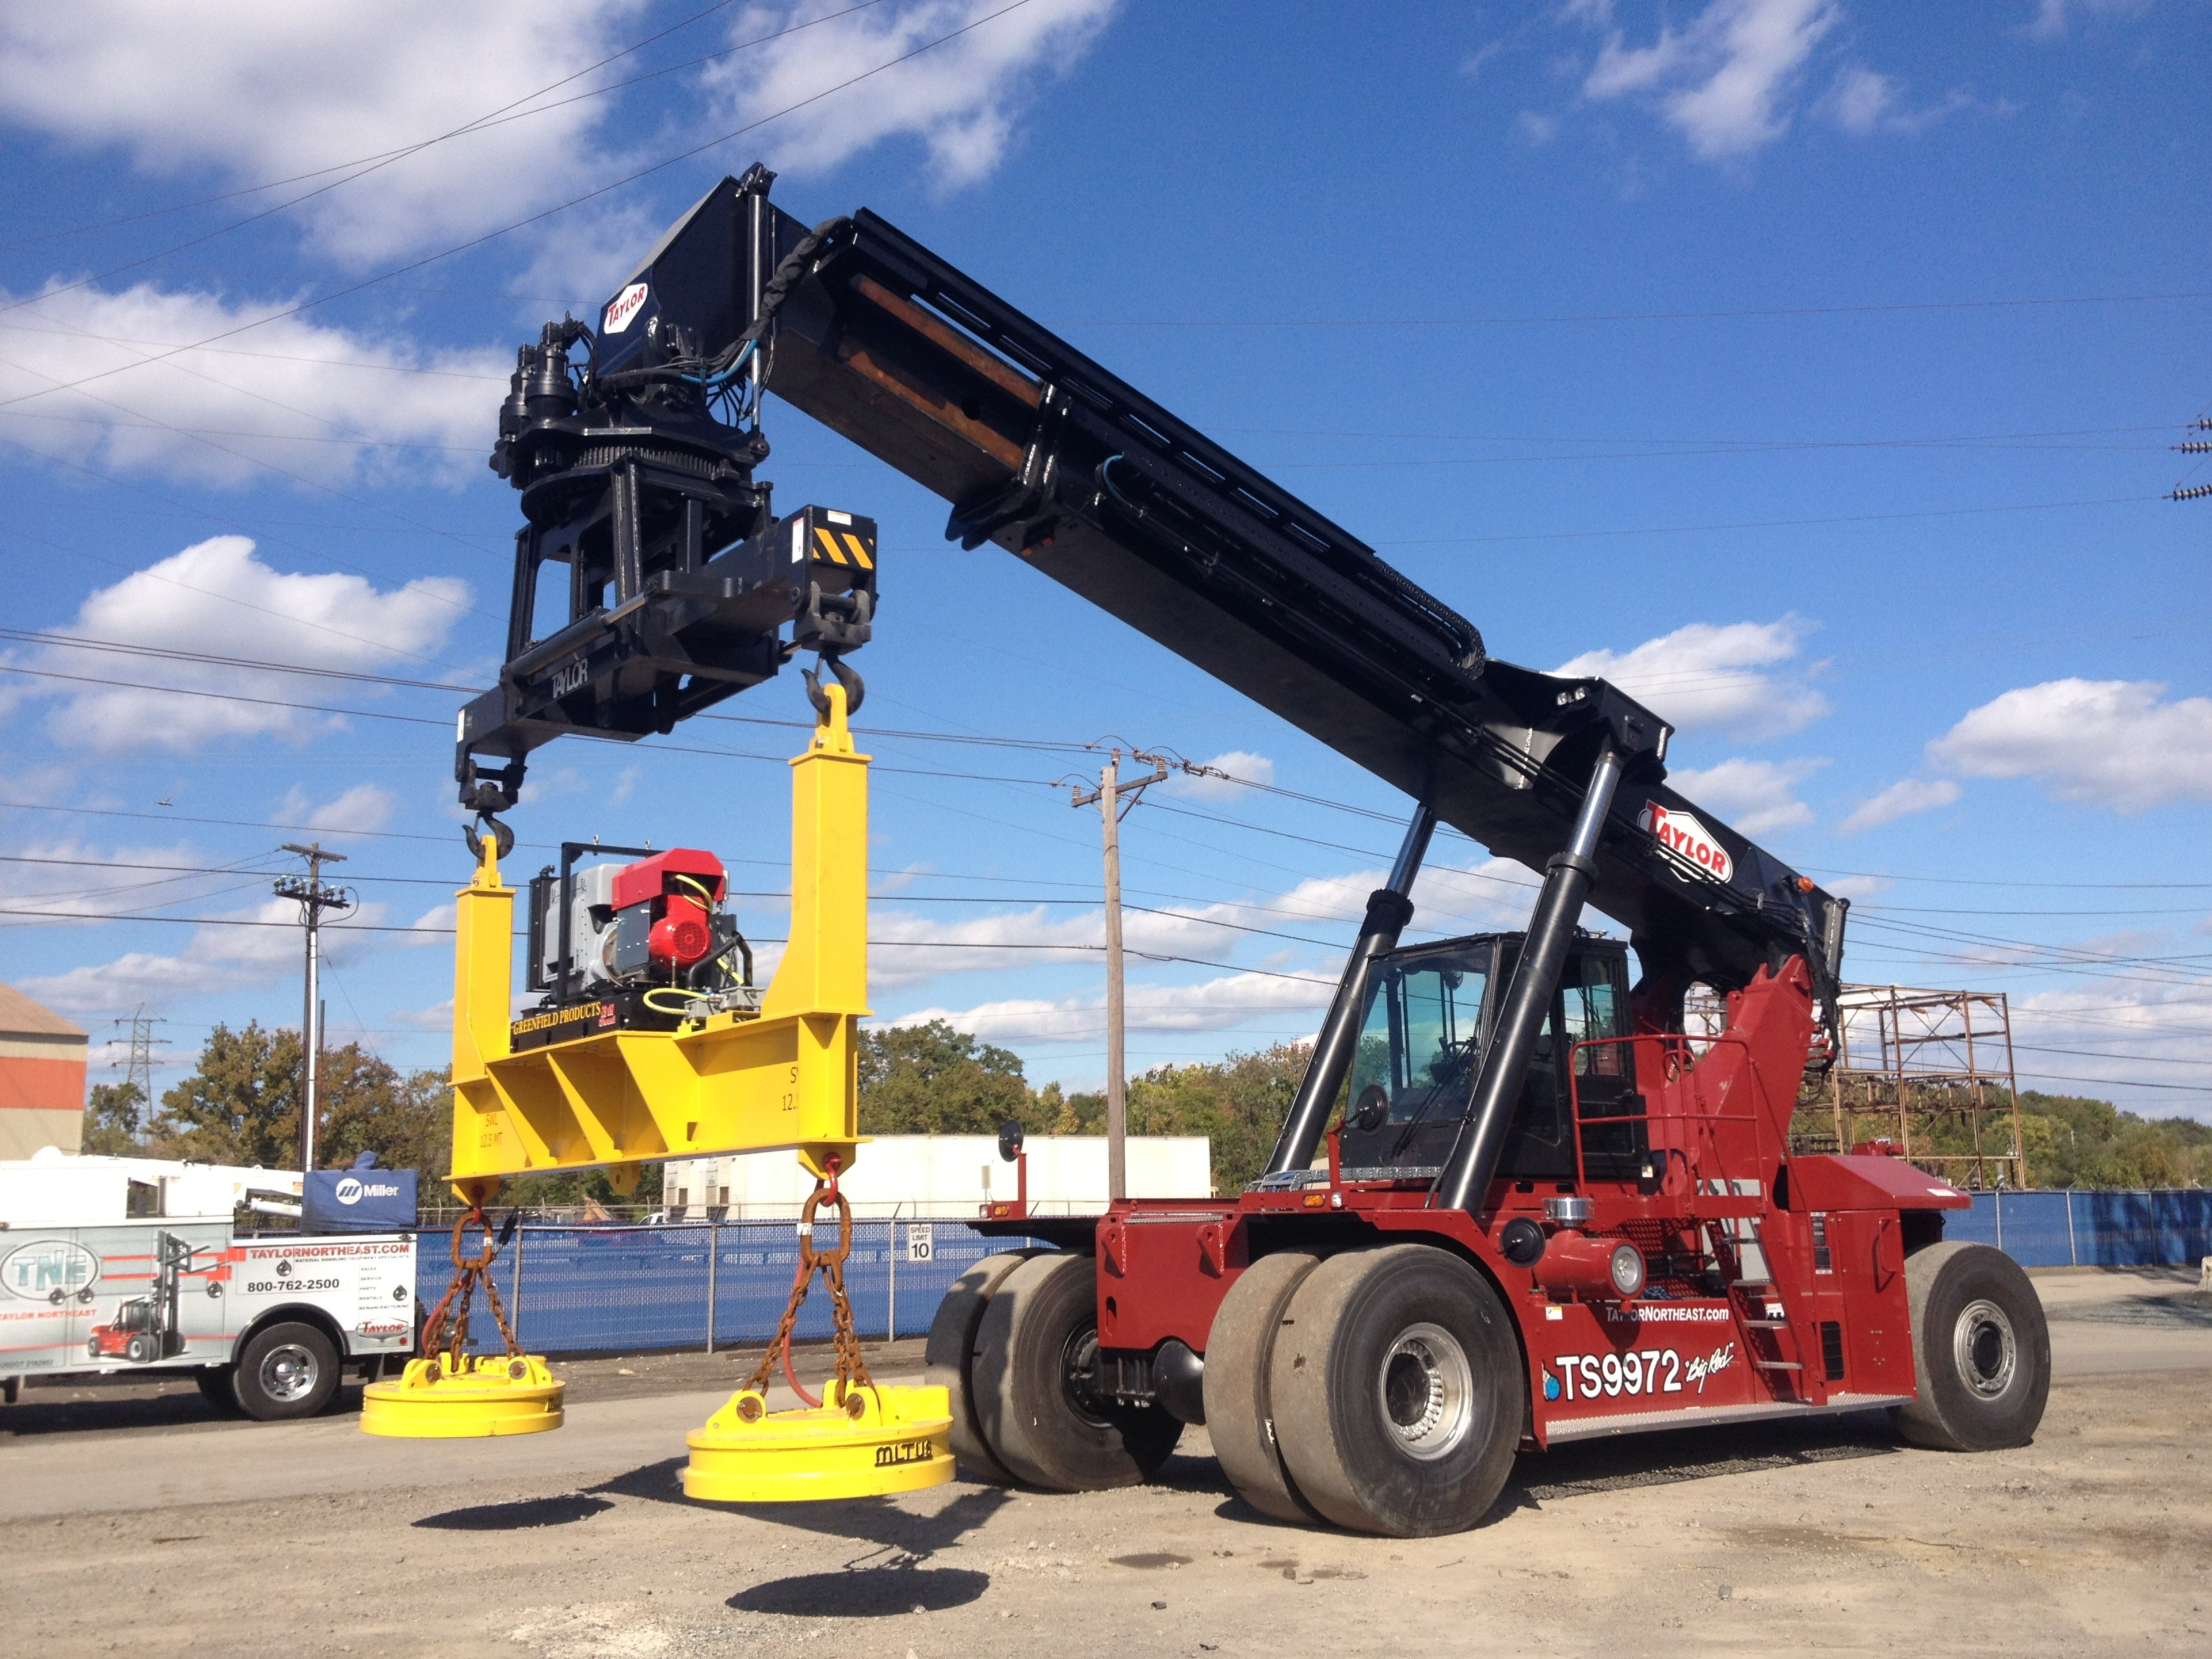
\includegraphics[width=0.5\textwidth]{figures/crane.jpg}
\caption{\label{fig:crane} An electromagnetic crane.}
\end{figure}
\end{frame}

\begin{frame}{Forces on Current-Carrying Conductors}
\textbf{Observe on board.} The force is $F = dl I B \sin\theta$, but $dl = Rd\theta$.
\begin{figure}
\centering
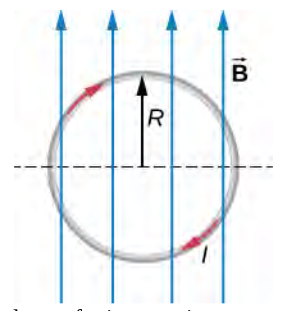
\includegraphics[width=0.4\textwidth,trim=0cm 0.1cm 0cm 0cm,clip=true]{figures/loop.png}
\caption{\label{fig:loop} Lorentz force on a loop of wire. Think of (a) the net force, and (b) the torque.  Which are non-zero?}
\end{figure}
\end{frame}

\begin{frame}{Forces on Current-Carrying Conductors}
\begin{figure}
\centering
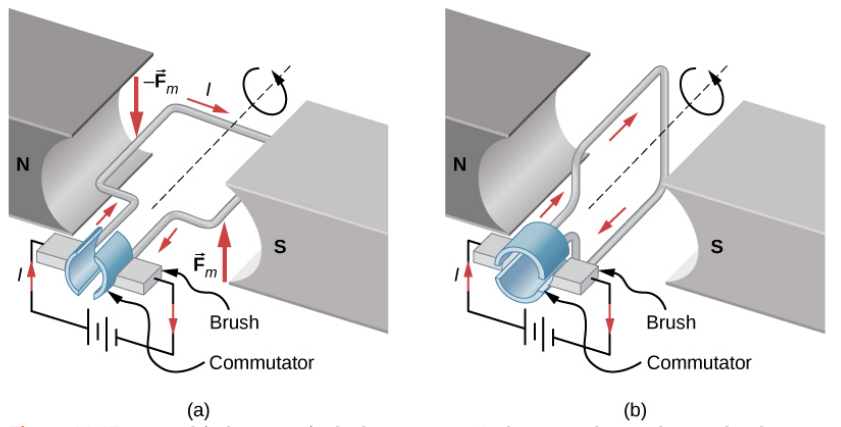
\includegraphics[width=0.7\textwidth]{figures/motor11.png}
\caption{\label{fig:loop2} Lorentz force on a loop of wire. Think of (a) the net force, and (b) the torque.  Which are non-zero?}
\end{figure}
\end{frame}

\begin{frame}{Forces on Current-Carrying Conductors}
\begin{figure}
\centering
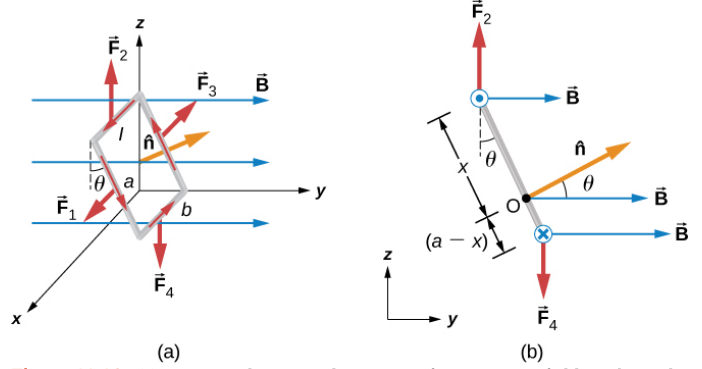
\includegraphics[width=0.7\textwidth]{figures/motor11_2.png}
\caption{\label{fig:loop3} The B-field causes a torque on a loop of current just like an E-field causes a torque on a dipole. We like to think of the \textbf{magnetic dipole moment} as $\vec{\mu} = NIA\hat{n}$.} \vspace{0.2cm}
\end{figure}
\end{frame}

\begin{frame}{Forces on Current-Carrying Conductors}
Let a single current loop of current $I$ and area $\vec{A} = A \hat{n}$ exist in a uniform magnetic field $\vec{B}$.  The torque $\tau$ on the loop is
\begin{equation}
\boxed{
\tau = \vec{\mu} \times \vec{B} \label{eq:torque}
}
\end{equation}
In Eq. \ref{eq:torque}, the quantity $\vec{\mu} = I\vec{A}$ is called the \textit{magnetic dipole moment.}
\begin{itemize}
\item $\vec{p} = q\vec{d}$ ... $\vec{\mu} = I\vec{A}$.
\item $\vec{\tau}_E = \vec{p} \times \vec{E}$ ... $\vec{\tau}_B = \vec{\mu} \times \vec{B}$
\end{itemize}
\textbf{How do we make a uniform $\vec{B}-field$?}...Postpone this to discuss one more effect: \textit{The Hall Effect}
\end{frame}

\section{The Hall Effect}

\begin{frame}{The Hall Effect}
Negative charge flows in conductors.
\begin{figure}
\centering
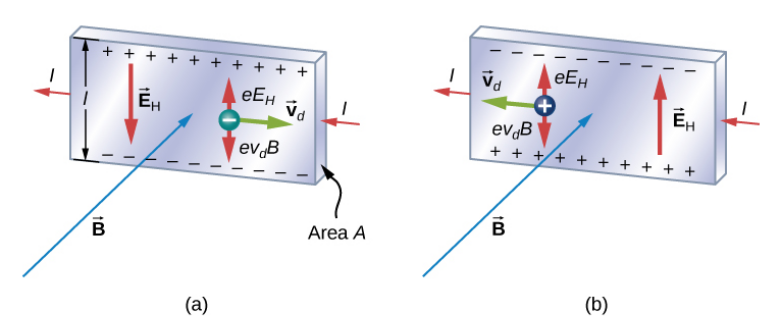
\includegraphics[width=0.7\textwidth]{figures/Hall.png}
\caption{\label{fig:Hall} The Hall effect is an important way to establish that what we call \textit{negative charge} is actually flowing in conductors.}
\end{figure}
\end{frame}

\begin{frame}{The Hall Effect}
Negative charge flows in conductors. \\ \vspace{0.5cm}
``Therefore, by simply measuring the sign of V, we can determine the sign of the majority charge carriers in a metal.
Hall potential measurements show that electrons are the dominant charge carriers in most metals. However, Hall potentials
indicate that for a few metals, such as tungsten, beryllium, and many semiconductors, the majority of charge carriers are
positive. It turns out that conduction by positive charge is caused by the migration of missing electron sites (called holes) on
ions.''
\end{frame}

\begin{frame}{The Hall Effect}
\small
\begin{figure}
\centering
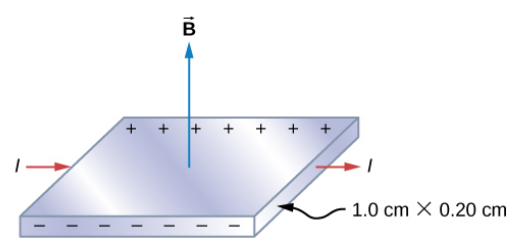
\includegraphics[width=0.6\textwidth]{figures/Hall2.png}
\caption{\label{fig:Hall2} An example of a Hall measurement, with some typical numbers.}
\end{figure}
\begin{itemize}
\item $I = 100$ A
\item $B = 1.5$ T
\item $l = 1.0\times 10^{-2}$ m
\item $n = 5.9 \times 10^{28}$ m$^{-3}$, $e = 1.6 \times 10^{-19}$ C
\item $A = 2.0 \times 10^{-5}$ m$^{2}$
\end{itemize}
\end{frame}

\begin{frame}{The Hall Effect}
\small
\begin{figure}
\centering
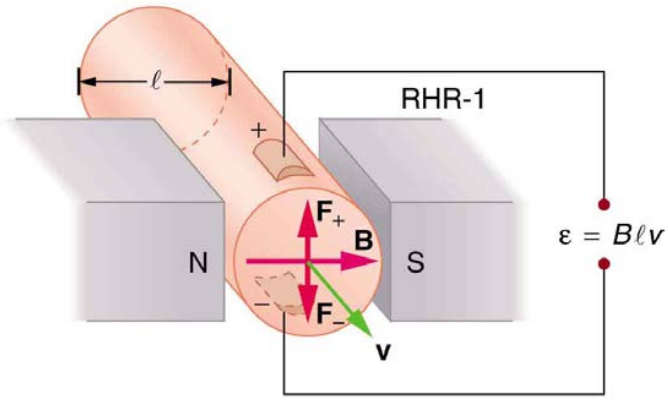
\includegraphics[width=0.45\textwidth]{figures/Hall3.png}
\caption{\label{fig:Hall3} A Hall measurement that is used to measure fluid flow.}
\end{figure}
\textbf{Group exercise:} A Hall effect flow probe is placed on an artery, applying a 0.1 T magnetic field across it, in a setup similar to that in Fig. \ref{fig:Hall3}. What is the blood velocity, given the vessel’s inside diameter is 4.00 mm and the Hall voltage is $0.8 \mu V$?
\end{frame}

\section{PHeT: Electromagnets}

\begin{frame}{PheT: Electromagnets}
Follow the link: \\ \vspace{0.5cm}
\url{https://phet.colorado.edu/en/simulation/magnets-and-electromagnets}
\end{frame}

\begin{frame}{PHeT: Electromagnets}
\small
\begin{enumerate}
\item Click on the electromagnet tab, and hide the field and compass using the menu in the upper right.  Also, display the magnetometer.
\item Place the magnetometer to one side of the \textit{solenoid.}  Work out the relationship between the magnetic field strength and voltage.  Is it linear, quadratic, or something else?
\item Assuming the circuit has some fixed resistance, is the relationship between current and field strength linear?  Why or why not?
\item Now fix the voltage and vary the number of loops.  Work out the relationship between magnetic field strength and loop number.  Is it linear, quadratic, or something else?
\item Propose an equation for $B_{solenoid}$ based on the prior measurements.
\end{enumerate}
\end{frame}

\begin{frame}{Force on a Moving Charges and Current Carrying Conductors}
\textbf{Electromagnets.}
\begin{figure}
\centering
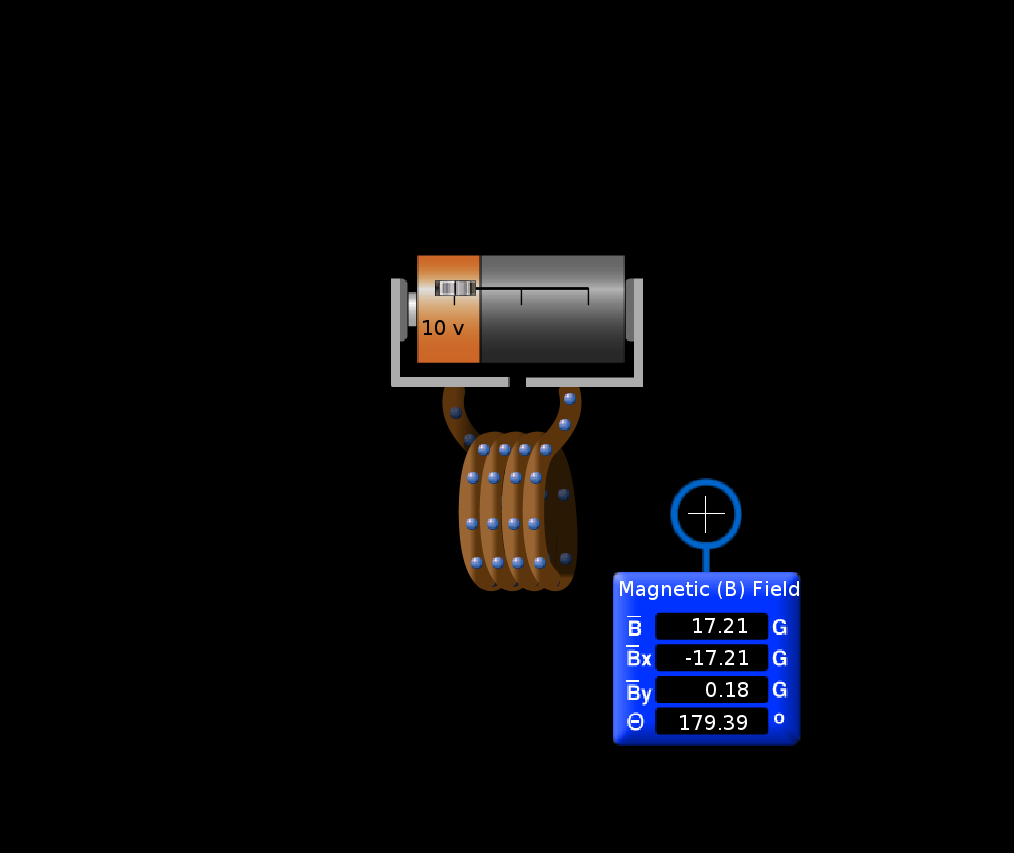
\includegraphics[width=0.55\textwidth]{figures/phetemmag.png}
\caption{\label{fig:phetemmag} The electromagnet converts charge to magnetic field strength.}
\end{figure}
\end{frame}

\begin{frame}{Force on a Moving Charges and Current Carrying Conductors}
The result should be something like:
\begin{align}
B &\propto N I \\
B &= \mu_0 n I
\end{align}
\begin{itemize}
\item $n$: Number of turns per unit length (because we can always change the density and get a different answer).
\item $I$: Current
\item $\mu_0$: Magnetic permeability of free space (solenoid is empty).
\end{itemize}
\end{frame}

\section{The Biot-Savart Law}

\begin{frame}{The Biot-Savart Law}
\begin{tcolorbox}[colback=white,colframe=black!40!black,title=The Biot-Savart Law]
\alert{Let a current $I$ exist along a line segment $d\vec{l}$ located a displacement $\vec{r}$ from an observation point.  The magnetic field contribution from this current element is
\begin{equation}
d\vec{B} = \frac{\mu_0}{4\pi} \frac{Id\vec{l} \times \hat{r}}{r^2}
\label{eq:biot}
\end{equation}}
\end{tcolorbox}
\begin{itemize}
\item Integrating this expression properly yields the total magnetic field at a given point
\item We have to take advantage of symmetries just like Coulomb's law
\end{itemize}
\end{frame}

\begin{frame}{The Biot-Savart Law}
\begin{figure}
\centering
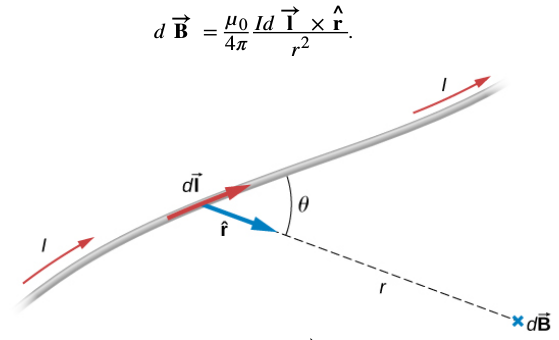
\includegraphics[width=0.55\textwidth]{figures/biot1.png}
\caption{\label{fig:biot1} The angle $\theta$ is between $\hat{r}$ and $d\vec{l}$, as shown.}
\end{figure}
\end{frame}

\begin{frame}{The Biot-Savart Law}
Which expression is equal to the magnitude of $Id\vec{l} \times \hat{r}$?
\begin{itemize}
\item A: $Idlr$
\item B: $Idlr\sin(\theta)$
\item C: $Idl\sin(\theta)$
\item D: $I\sin(\theta)$
\end{itemize}
\end{frame}

\begin{frame}{The Biot-Savart Law}
If the B-field due to a line-segment of current is 1.0 Gauss at 1cm, what is the value of the B-field 10 cm from the line-segment, for the same orientation?
\begin{itemize}
\item A: 0.1 Gauss
\item B: 0.05 Gauss
\item C: 1.0 Gauss
\item D: 0.01 Gauss
\end{itemize}
\end{frame}

\begin{frame}{The Biot-Savart Law}
If the B-field due to a line-segment of current is 1.0 Gauss at 1cm, and $\hat{r}$ is perpendicular to $d\vec{l}$, what is the B-field when $d\vec{l}$ is \textit{parallel} to $d\vec{l}$?
\begin{itemize}
\item A: 0.0 Gauss
\item B: 0.05 Gauss
\item C: 1.0 Gauss
\item D: 0.01 Gauss
\end{itemize}
\end{frame}

\begin{frame}{The Biot-Savart Law}
If the B-field due to a line-segment of current is 1.0 Gauss for a current of 0.5 A, what is the B-field when the current is increased to 1.0 A?
\begin{itemize}
\item A: 0.0 Gauss
\item B: 0.02 Gauss
\item C: 2.0 Gauss
\item D: 0.02 Gauss
\end{itemize}
\end{frame}

\begin{frame}{The Biot-Savart Law}
If the B-field due to a line-segment of current is 1.0 Gauss for a current of 0.5 A at a distance of 10 cm, what is the B-field when the current is increased to 1.0 A, and the distance is decreased to 1 cm?
\begin{itemize}
\item A: 20 Gauss
\item B: 200 Gauss
\item C: 500 Gauss
\item D: 1000 Gauss
\end{itemize}
\end{frame}

\section{Biot-Savart Example: The thin straight wire}

\begin{frame}{Biot-Savart Example: The thin straight wire}
\begin{figure}
\centering
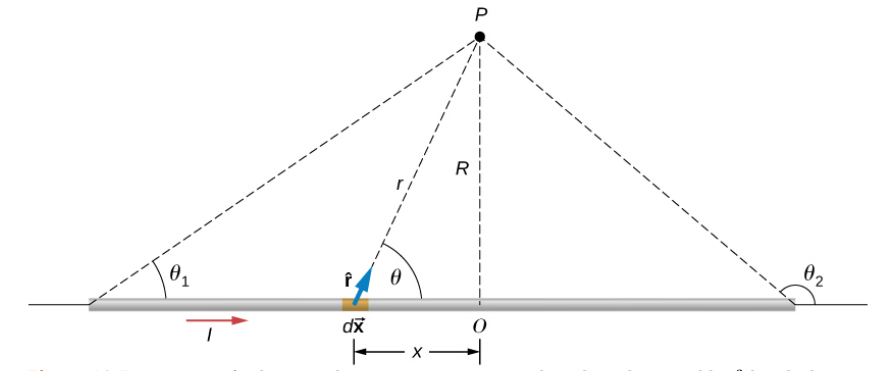
\includegraphics[width=0.75\textwidth]{figures/biot2.png}
\caption{\label{fig:biot2} Observe on board the derivation of the formula for $\vec{B}$ at a point $P$.}
\end{figure}
\end{frame}

\begin{frame}{Biot-Savart Example: The thin straight wire}
The magnetic field a distance R from a long thin straight wire carrying current I is
\begin{equation}
\vec{B} = \frac{\mu_0 I}{2\pi R} \hat{\phi}
\end{equation}
The direction is in a right-handed sense around the wire.
\end{frame}

\begin{frame}{Biot-Savart Example: The three straight wires}
\begin{figure}
\centering
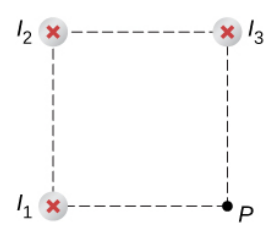
\includegraphics[width=0.3\textwidth]{figures/biot3.png}
\caption{\label{fig:biot3} Derive the magnitude and direction for $\vec{B}$ at a point $P$, if the sides of the square are 1cm and the currents are each 2.0 A.}
\end{figure}
\end{frame}

\section{Biot-Savart Example: The current loop}

\begin{frame}{Biot-Savart Example: The thin straight wire}
\begin{figure}
\centering
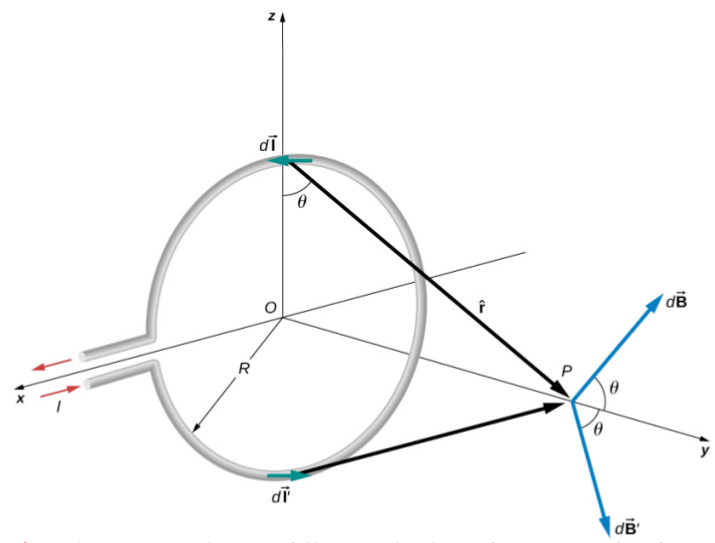
\includegraphics[width=0.75\textwidth]{figures/magloop.png}
\caption{\label{fig:biot4} Observe on board the derivation of the formula for $\vec{B}$ at a point $P$.}
\end{figure}
\end{frame}

\begin{frame}{Biot-Savart Example: The three straight wires}
Let a current loop with magnetic moment $\vec{\mu}$ and radius $R$ carry a current I.  The B-field along the loop axis at a distance $y$ from the center is
\begin{equation}
\vec{B} = \frac{\mu_0 \vec{\mu}}{2\pi(y^2+R^2)^{3/2}}
\end{equation}
At the center of the loop, the field simplifies to
\begin{equation}
\vec{B}_{center} = \frac{\mu_0 I}{2 R}\hat{\mu}
\end{equation}
\end{frame}

\begin{frame}{Biot-Savart Example: The current loop}
Let a current loop be oriented in the x-y plane, with the current proceding counter-clockwise as we look down on it from positive z positions.  In which direction does the magnetic moment point?
\begin{itemize}
\item A: $-\hat{z}$
\item B: $\hat{y}$
\item C: $\hat{z}$
\item D: in x-y plane
\end{itemize}
\end{frame}

\begin{frame}{Biot-Savart Example: The current loop}
The current is 0.5 A, the radius is 2 cm.  What is the B-field magnitude at the center of the loop?
\begin{itemize}
\item A: 0.16 Gauss
\item B: 1.6 Gauss
\item C: 0.016 Tesla
\item D: 1.6 Tesla
\end{itemize}
\end{frame}

\begin{frame}{Biot-Savart Example: The current loop}
Two identical current loops are oriented with centers at $x=y=0$, but with different z values.  If the currents spin in opposite directions, which of the following is true of the B-field at a point half-way between the loop centers?
\begin{itemize}
\item A: It points in the $+\hat{z}$ direction
\item B: It points in the $-\hat{z}$ direction
\item C: It points in the $+\hat{y}$ direction
\item D: It is 0.0 T
\end{itemize}
\end{frame}

\section{Lab Activity: The First Electromagnet}

\begin{frame}{Lab Activity: The First Electromagnet}
\begin{figure}
\centering
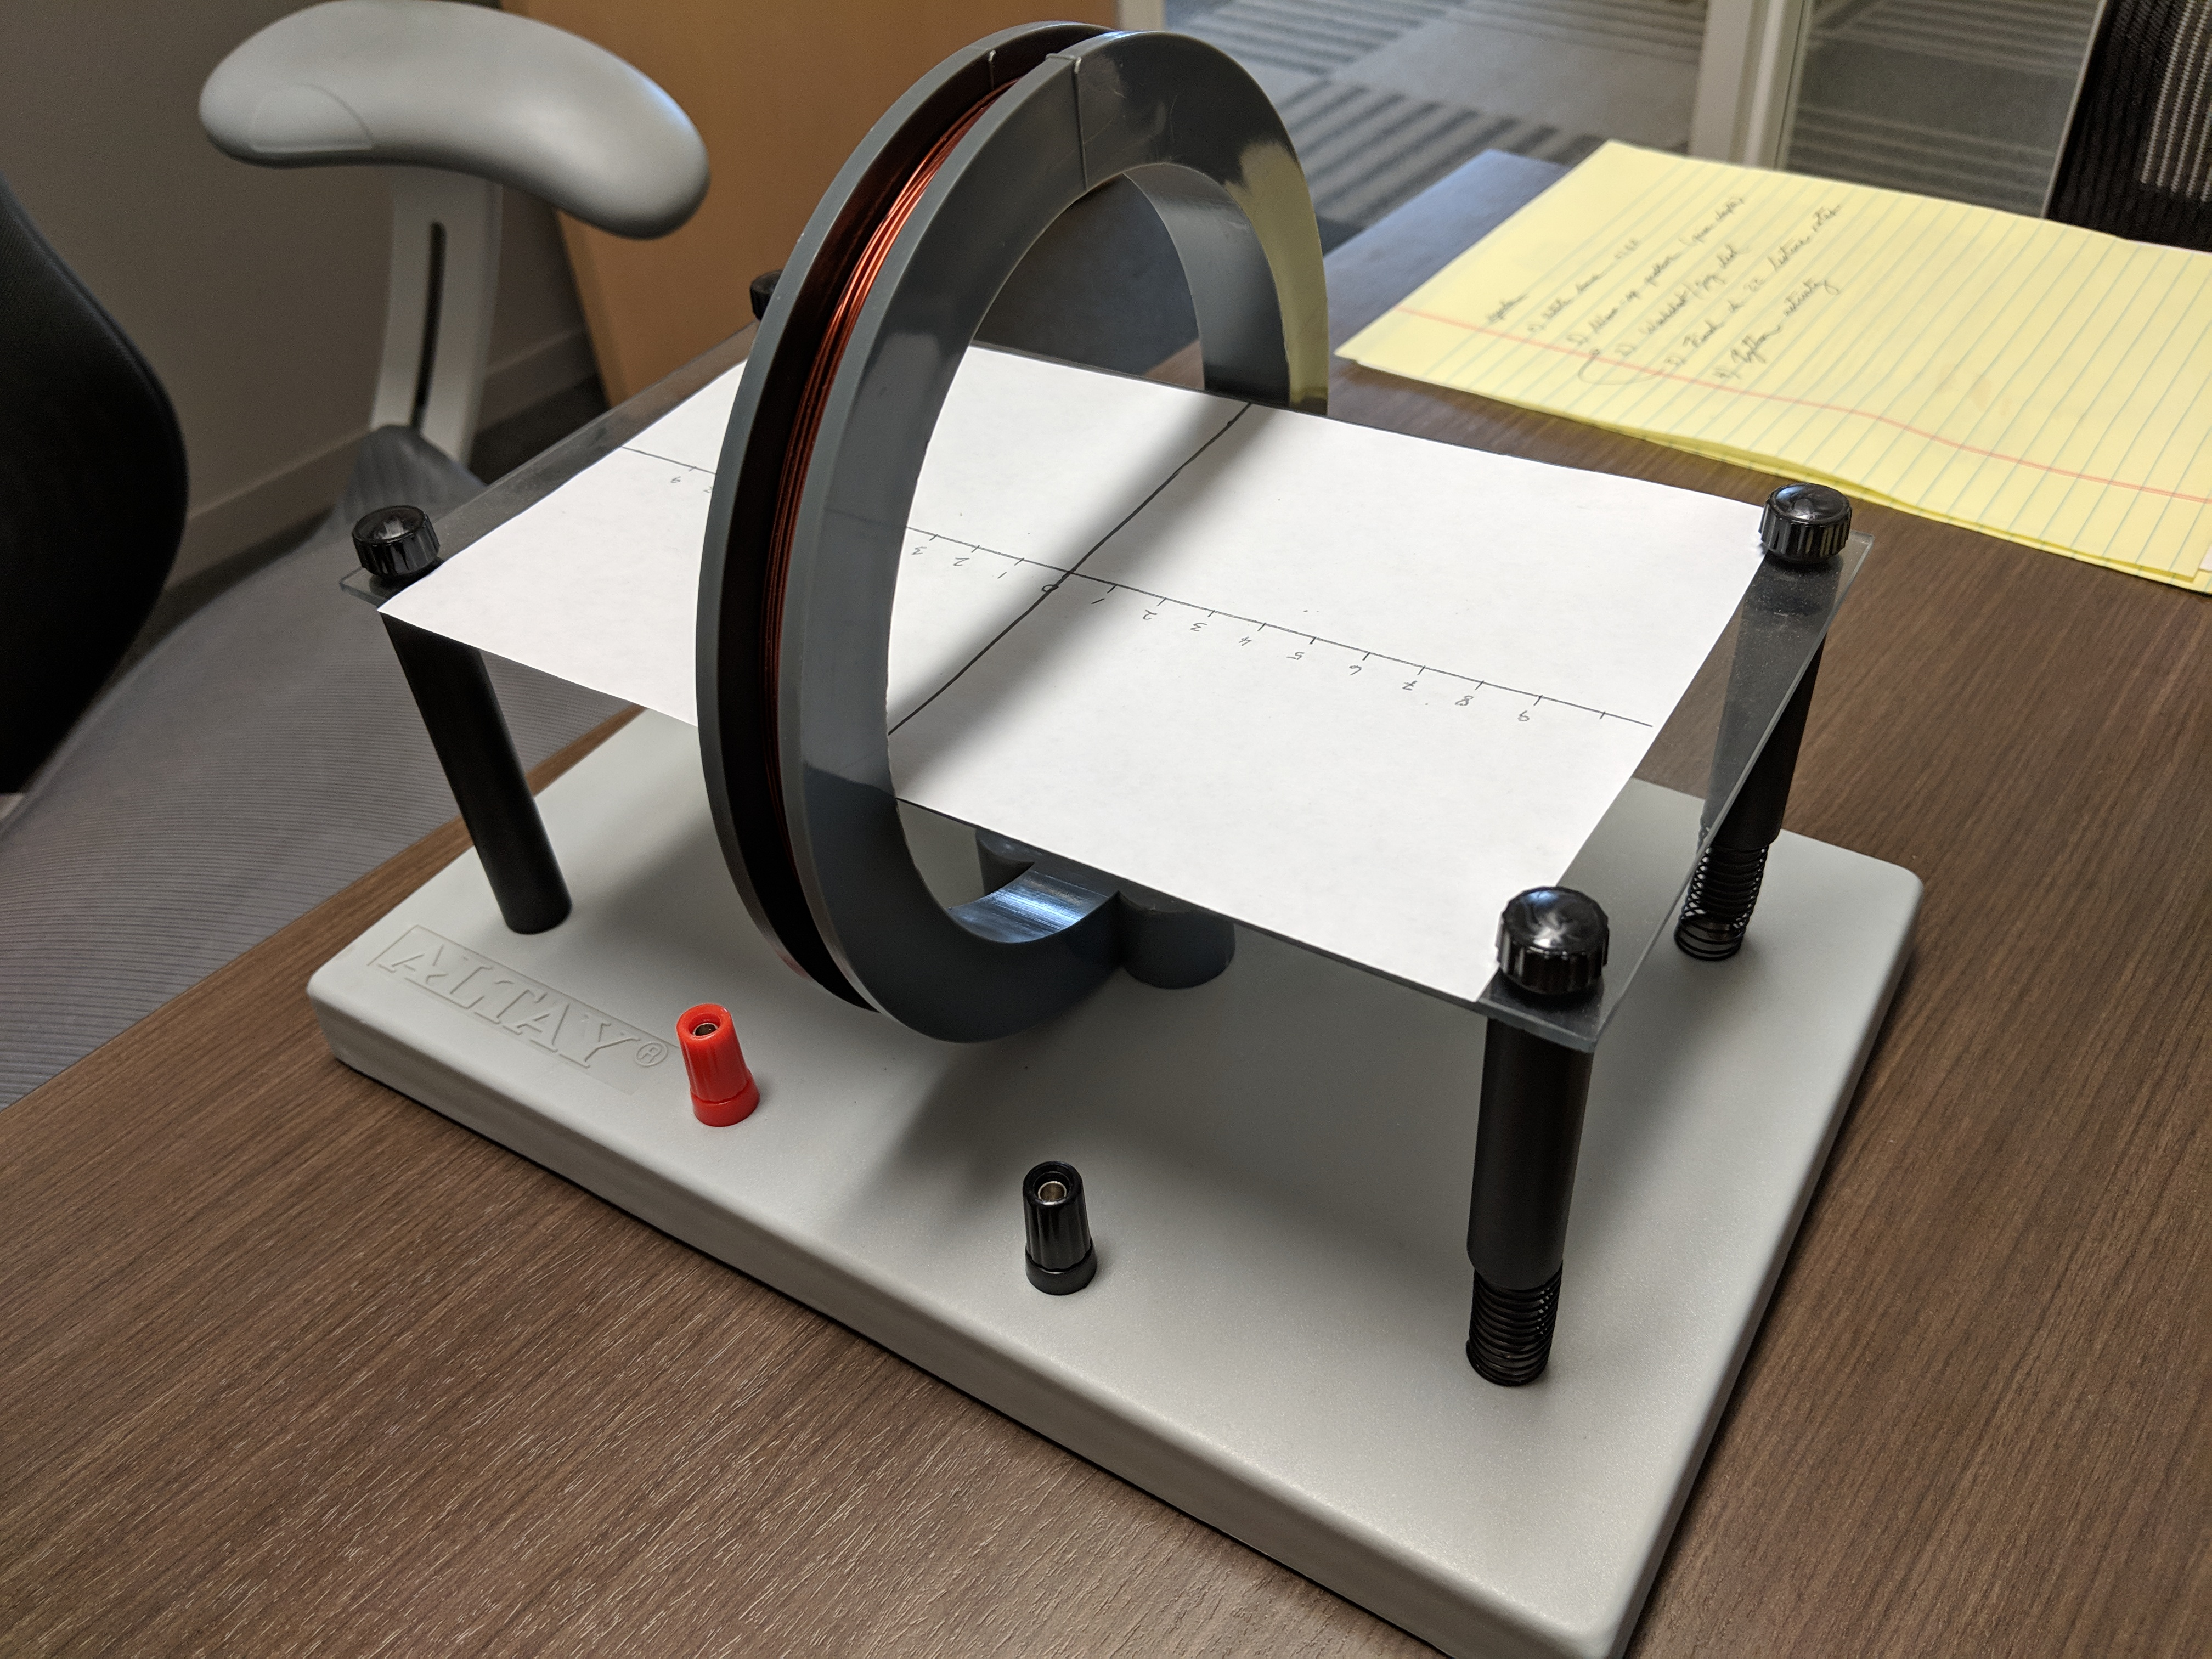
\includegraphics[width=0.75\textwidth]{figures/coil.jpg}
\caption{\label{fig:lab1coil} The electromagnetic coil has $N$ turns, and we must figure out how many.  Which formula is appropriate for describing the magnetic field at the center?}
\end{figure}
\end{frame}

\begin{frame}{Lab Activity: The First Electromagnet}
\textbf{Parts required:}
\begin{enumerate}
\item Vernier LabPro and magnetic probe attachment
\item Desktop PC with Logger Pro
\item DC power supply (\textbf{current limiting})
\item Red/black cables
\item Electromagnetic coil with platform
\item Ruler
\end{enumerate}
\end{frame}

\begin{frame}{Lab Activity: The First Electromagnet}
\textbf{Instructions:}
\begin{enumerate}
\item Connect the Vernier LabPro to the PC, and the magnetic probe to the LabPro.
\item Launch the LoggerPro program (should be an icon on the Desktop)
\item LoggerPro should recongnize the instrument and begin displaying magnetic field in mT (lower left)
\item Record average magnetic field in 6 direction ($\pm x$, $\pm y$, $\pm z$ with respect to coil).  Let the z-axis be aligned with the magnetic moment of the coil. Assess the uncertainty in each direction.
\item Use the ruler to measure the radius of the coils. Assess the uncertainty.
\end{enumerate}
\end{frame}

\begin{frame}{Lab Activity: The First Electromagnet}
\textbf{Instructions:}
\begin{enumerate}
\item The DC power supply has two black knobs: voltage and current.
\item The current knob controls the maximum current that can flow from the terminals.
\item Connect the power supply to the coil with the red and black cables, and turn down the current knob until it reads between 0.1-0.6 amps.
\item Use the magnetic probe to measure the magnetic field at the center of the coils.  How many turns $N$ are in the coil?
\item Make a plot of B-field versus current.  You can fit the slope in Excel in the usual way (ask if this is unfamiliar).
\end{enumerate}
\end{frame}

\begin{frame}{Lab Activity: The First Electromagnet}
\textbf{Instructions:}
\begin{enumerate}
\item Using the slope of B vs. I, derive a more precise measurement of the turns $N$ in the coil.
\item Is there a \textit{systematic error} in the slope method?  When is B-field zero?
\item We will need this number in subsequent labs!
\end{enumerate}
\end{frame}

\section{Amp\`{e}re's Law}

\begin{frame}{Amp\`{e}re's Law}
\begin{tcolorbox}[colback=white,colframe=black!40!black,title=Amp\`{e}re's Law]
\alert{Let $I$ be the total current passing through any open surface S whose perimeter is a closed path of integration:
\begin{equation}
\oint \vec{B} \cdot d\vec{l} = \mu_0 I_{\rm enc}
\label{eq:ampereslaw}
\end{equation}}
\end{tcolorbox}
\begin{itemize}
\item Compare to Gauss' Law for charge
\item The left-hand side is always 0 for E-fields
\item See online tutorial for derivation
\end{itemize}
\end{frame}

\begin{frame}{Amp\`{e}re's Law}
\begin{figure}
\centering
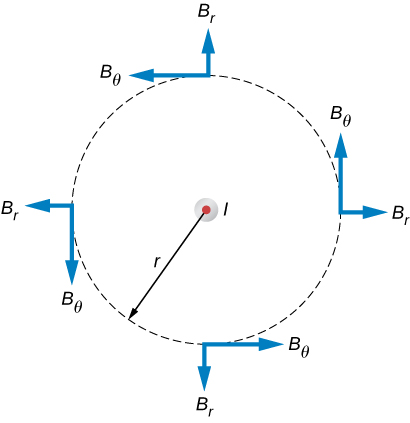
\includegraphics[width=0.5\textwidth]{figures/amplaw1.jpeg}
\caption{\label{fig:amplaw1} Directions for a right-handed B-field around a current emerging from the page.}
\end{figure}
\end{frame}

\begin{frame}{Amp\`{e}re's Law}
Which of the following is the correct formula for the B-field magnitude a distance $r$ from a long thin straight wire?
\begin{itemize}
\item A: $B = \frac{\mu_0 I}{2\pi r^2}$
\item B: $B = \frac{\mu_0 I}{2\pi}$
\item C: $B = \frac{\mu_0}{2\pi r}$
\item D: $B = \frac{\mu_0 I}{2\pi r}$
\end{itemize}
\end{frame}

\begin{frame}{Amp\`{e}re's Law}
Suppose we form an Amperian loop around a current I that flows in the $\hat{k}$ direction, and another current I that flows in the $-\hat{k}$ direction.  Which of the following is true of the integrated B-field around the loop? (Assume that $\hat{k}$ comes out of the page).
\begin{itemize}
\item A: There's current in the loop, so B > 0
\item B: There's negative current i the loop, so B < 0
\item C: The currents cancel, so B = 0
\item D: Since the loop is a distance $r$ away from the currents, the B-field is small.
\end{itemize}
\end{frame}

\begin{frame}{Amp\`{e}re's Law}
Suppose we form an Amperian loop around a current I that flows in the $\hat{k}$ direction, and another current I that flows in the $-\hat{k}$ direction.  Which of the following is true of the integrated B-field around the loop? (Assume that $\hat{k}$ comes out of the page).
\begin{itemize}
\item A: There's current in the loop, so B > 0
\item B: There's negative current i the loop, so B < 0
\item C: The currents cancel, so B = 0
\item D: Since the loop is a distance $r$ away from the currents, the B-field is small.
\end{itemize}
\end{frame}

\begin{frame}{Amp\`{e}re's Law}
\begin{columns}[T]
\begin{column}{0.5\textwidth}
\small
Which of the following Amperian loops causes the quantity $\oint \vec{B} \cdot d\vec{l}$ to be positive?
\begin{itemize}
\item A: A and B
\item B: A and C
\item C; B and D
\item D: B and C
\end{itemize}
\end{column}
\begin{column}{0.5\textwidth}
\begin{figure}
\centering
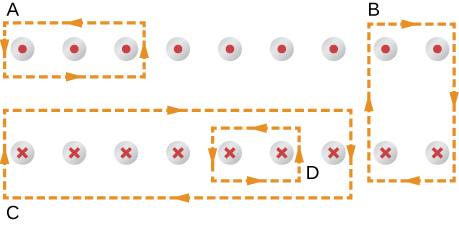
\includegraphics[width=0.95\textwidth]{figures/ampQuestion1.jpeg}
\caption{\label{fig:ampQuestion1} A cross-section of a coil of wire with four Amperian loops.}
\end{figure}
\end{column}
\end{columns}
\end{frame}

\begin{frame}{Amp\`{e}re's Law}
\begin{columns}[T]
\begin{column}{0.5\textwidth}
\small
If the currents are all I in Fig. \ref{fig:ampQuestion2}, what is the value of $\oint \vec{B} \cdot d\vec{l}$ for loop D?
\begin{itemize}
\item A: $\mu_0 I$
\item B: $-\mu_0 I$
\item C; $2\mu_0 I$
\item D: $-2\mu_0 I$
\end{itemize}
\end{column}
\begin{column}{0.5\textwidth}
\begin{figure}
\centering
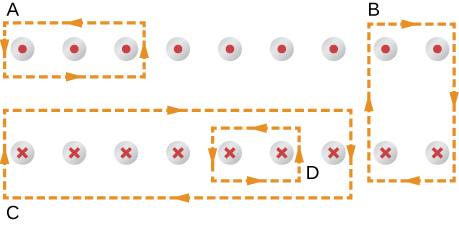
\includegraphics[width=0.95\textwidth]{figures/ampQuestion1.jpeg}
\caption{\label{fig:ampQuestion2} A cross-section of a coil of wire with four Amperian loops.}
\end{figure}
\end{column}
\end{columns}
\end{frame}

\begin{frame}{Amp\`{e}re's Law}
\begin{columns}[T]
\begin{column}{0.5\textwidth}
\small
If the currents are all I in Fig. \ref{fig:ampQuestion3}, what is the value of $\oint \vec{B} \cdot d\vec{l}$ for loop B?
\begin{itemize}
\item A: $4\mu_0 I$
\item B: $-4\mu_0 I$
\item C; $\mu_0 I$
\item D: $0$
\end{itemize}
\end{column}
\begin{column}{0.5\textwidth}
\begin{figure}
\centering
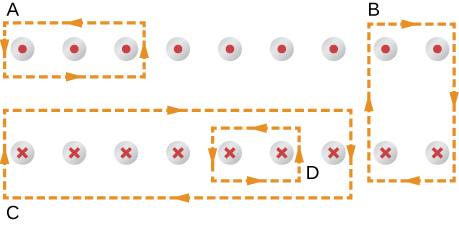
\includegraphics[width=0.95\textwidth]{figures/ampQuestion1.jpeg}
\caption{\label{fig:ampQuestion3} A cross-section of a coil of wire with four Amperian loops.}
\end{figure}
\end{column}
\end{columns}
\end{frame}

\begin{frame}{Amp\`{e}re's Law}
\begin{columns}[T]
\begin{column}{0.5\textwidth}
\small
In Fig. \ref{fig:ampQuestion4}, which setup has the \textit{most negative} value for $\oint \vec{B} \cdot d\vec{l}$ ?
\begin{itemize}
\item A: (a)
\item B: (b)
\item C; (c)
\item D: (d)
\item E: (e)
\end{itemize}
\end{column}
\begin{column}{0.5\textwidth}
\begin{figure}
\centering
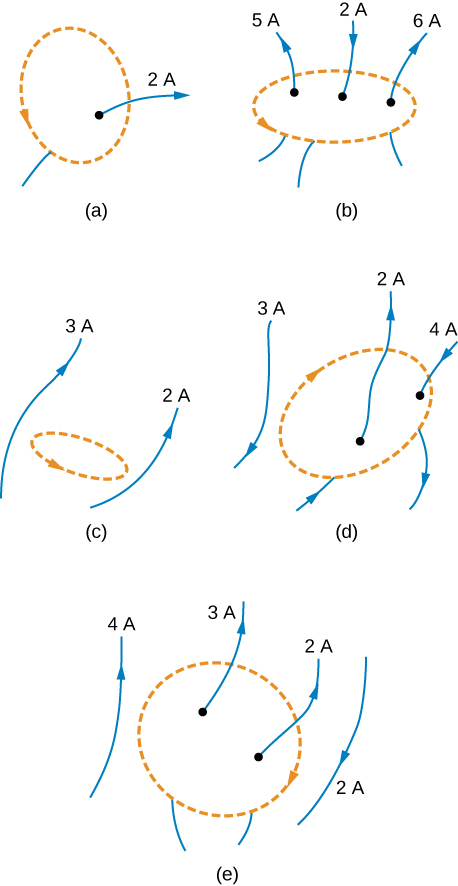
\includegraphics[width=0.55\textwidth]{figures/ampQuestion2.jpeg}
\caption{\label{fig:ampQuestion4} Currents and Amperian loops.}
\end{figure}
\end{column}
\end{columns}
\end{frame}

\begin{frame}{Amp\`{e}re's Law}
What will be the B-field within and outside of a wire if we account for the thickness of the wire?
\begin{figure}
\centering
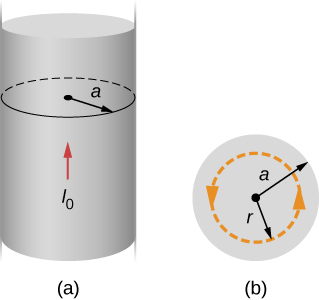
\includegraphics[width=0.5\textwidth]{figures/amplaw2.jpeg}
\caption{\label{fig:amplaw2} A wire with some thickness $a$, and a current $I_0$ uniformly distributed.}
\end{figure}
\end{frame}

\begin{frame}{Amp\`{e}re's Law}
What will be the B-field within and outside of a wire if we account for the thickness of the wire? \alert{Demonstration:}
\begin{itemize}
\item Current density: $\int \vec{J} \cdot d\vec{A} = I$
\item Amperian loop orientation, and enclosed current
\item Perform the integral
\item Graph the B-field
\end{itemize}
\end{frame}

\section{Summary}

\begin{frame}{Unit 3 Summary}
\textbf{Reading: Chapter 11 and 12}
\begin{enumerate}
\item Magnetism and magnetic fields
\item Motion of a charged particle in a magnetic field
\item Forces on conductors carrying current
\item Current loops
\item The Hall effect
\item Applications
\item Amp\`{e}re's Law
\end{enumerate}
\end{frame}

\end{document}
